% siminos/CLE/movingFrames.tex
% $Author: siminos $ $Date: 2009-12-19 02:59:14 +0100 (Sat, 19 Dec 2009) $

The \mframes, introduced by G. Darboux and systematized by \'E. Cartan\rf{CartanMF},
can be thought of as generalization of the Frenet-Serret comoving frame.
The \Mframes\ can be used to generate functionally independent invariant coordinates
for the action of a group $\Group$ on a manifold $\Manif$ under
very general assumptions.  Here we will describe how, and to what extend,
the invariants thus generated can be utilized for symmetry reduction in 
high-dimensional flows. Our presentation draws from the reformulation of the \mframes\ 
by Fels and Olver\rf{FelsOlver98,FelsOlver99} but our emphasis is on the implementation
of the method as a geometrical, and therefore linear, operation that can be efficiently
implemented even in higher-dimensional flows, rather than in the explicit 
determination of invariant functions as in \refref{FelsOlver98,FelsOlver99}. 

The main idea behind \mframes\ is that we can, at least locally, 
map each point along any solution $\ssp(\tau)$ to a unique 
representative $\sspRed(\tau)$ of the associated
group orbit equivalence class, by a suitable rotation
\beq
\ssp(\tau) = \LieEl(\tau) \, \sspRed(\tau)
\,.
\ee{EquiTraj}
Equivariance implies the two points are equivalent.
In the `\mframes' the \reducedsp\ representative $\sspRed$
of a group orbit equivalence class is picked by slicing across the group orbits
by a fixed hypersurface.
%
%%%%%%%%%%%%%%%%%%%%%%%%%%%%%%%%%%%%%%%%%%%%%%%%%
\begin{figure}[h]
\begin{center}
 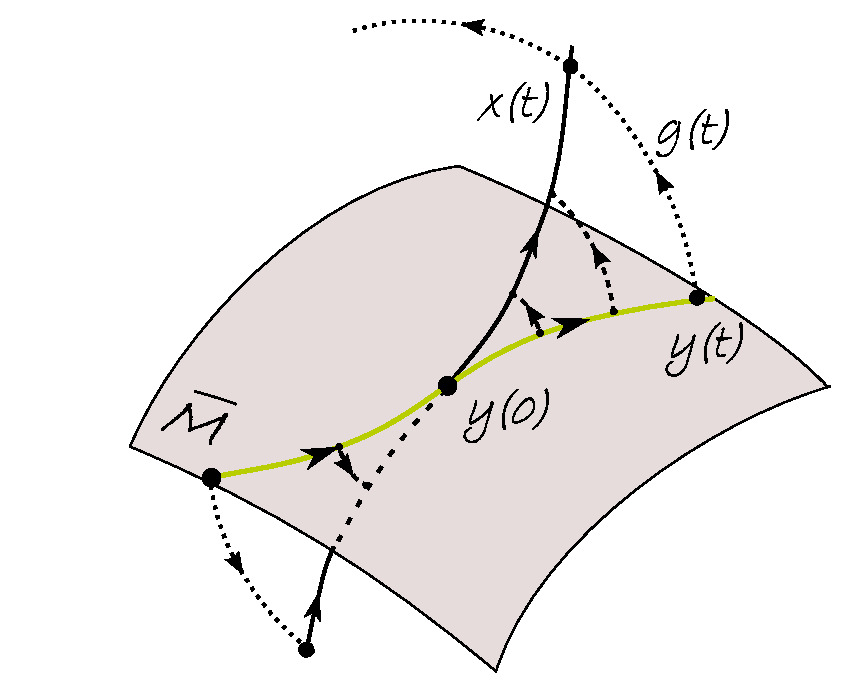
\includegraphics[width=0.5\textwidth]{../figs/ReducTraj}
\end{center}
\label{fig:ReducTraj}
\caption{
\Slice\ \pSRed\ is a Poincar\'e section \refeq{PCsectQ} for
group orbits (indicated by dotted lines here). The full
\statesp\ trajectory $\ssp(t)$ and and the \reducedsp\
trajectory $\sspRed(t)$ belong to the same group orbit
$\pS_{\ssp(t)}$ and are equivalent up to a group rotation
$\LieEl(t)$ \refeq{EquiTraj}.
}
\end{figure}
%%%%%%%%%%%%%%%%%%%%%%%%%%%%%%%%%%%%%%%%%%%%%%%%%%
%
\ES{move elsewhere: We start by describing how the
method works for a finite segment of the full \statesp\
trajectory.}

In the following it will be useful to introduce the
notion of a \emph{\slice}, an $(n-r)$-dimensional submanifold $K$
of $\Manif$ such that $K$ intersects all group orbits in an
open neighborhood of $\ssp \in K$ transversally and at most once. 
In other words, `\slice' is a Poincar\'e section
for group orbits. As is the case for the dynamical Poincar\'e sections,
in general a single \slice\ does not suffice to intersect all
group orbits of points in \pS. Fels and Olver\rf{FelsOlver99}
call a manifold $K$ that intersects \emph{all} group orbits a
\emph{regular cross-section}, and refer to a \slice\ as a local
cross-section. Here we prefer the term slice
to cross-section as the latter has a well established usage in the physics
literature.

Loosely speaking, one can construct a local {\csection} passing
through any point $x\in \Manif$ if the group orbits of \Group\
have the same dimension, \ie\ away from {\fixedsp s}
of continuous subgroups of \Group, see \refref{FelsOlver99} for
details.

The simplest {\em \slice\ condition} defines a linear \slice\ as a
$(d\!-\!N)$-dim\-ens\-ion\-al hyperplane \pSRed\ normal to
the $N$ group rotation tangents $\sliceTan{a}$ at point $\slicep$:
\beq
(\sspRed - \slicep )^T \sliceTan{a} =0
    \,,\qquad
\sliceTan{a} = \groupTan_a(\slicep) = \Lg_a \, \slicep
\,.
\ee{PCsectQ}

%%%%%%%%%%%%%%%%%%%%%%%%%%%%%%%%%%%%%%%%%%%%%%%%%%
% computed by PCunrot.nb, then hand-drawn
% by dasbuch/book/FigSrc/xfig/PCunrot.fig
% then branched to dasbuch/book/FigSrc/xfig/ESunrot.fig
\begin{figure}
 \begin{center}
  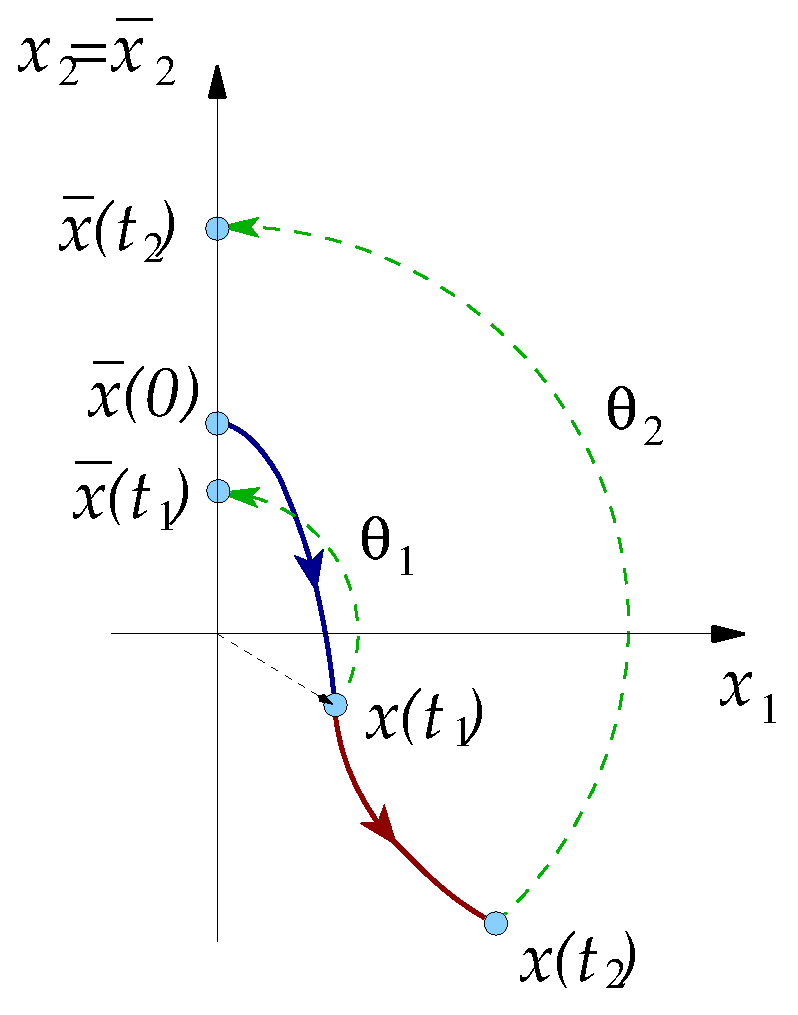
\includegraphics[width=0.5\textwidth]{../figs/ESunrot}
 \end{center}
 \label{fig:ESunrot}
 \caption{\Mframes\ for a flow $\SOn{2}$-equivariant under
\refeq{CLfRots} with \slice\ through $\slicep=(0,1,0,0,0)$,
group tangent $\sliceTan{}=(1,0,0,0,0)$. The clockwise
orientation condition restricts the \slice\ to half-hyperplane
$\sspRed_1=0,\;\sspRed_2>0$. A trajectory started on the
\slice\ at $\sspRed(0)$, evolves to a \statesp\ point with a
non-zero $\ssp_1(t_1)$. Compute the polar angle $\gSpace_1$
of $\ssp(t_1)$ in the $(\ssp_1,\ssp_2)$ plane. Rotate $\ssp(t_1)$
clockwise by $\gSpace_1$ to $\sspRed(t_1) =
\LieEl(-\gSpace_1)\,\ssp(t_1)$, so that the equivalent point
on the circle lies on the \slice, $\sspRed_1(t_1) =0$. Repeat
for all sample points $\ssp(t_i)$ along the trajectory.}
\end{figure}
%%%%%%%%%%%%%%%%%%%%%%%%%%%%%%%%%%%%%%%%%%%%%%%%%%


\ES{repeated?: In the following let $\Group$ be $N$-dimensional and act on a
$d$-dimensional manifold $\Manif$.}
\ES{dropped: Assume that for a given $\ssp\in\pS$ and a given \slice\
$\pSRed$ there exists} 

For group orbits intersected by a slice we can identify the unique group element
$\LieEl=\LieEl(\ssp)$ that rotates $\ssp$ into the slice,
$\LieEl\ssp = \sspRed \in \pSRed$. The map that
associates to a \statesp\ point $\ssp$ a Lie group action
$\LieEl(\ssp)$ is called a \emph{moving frame}. \Mframes\ 
can be interpreted as a change of variables
\beq
\sspRed = \LieEl^{-1} \, \ssp
\,,
\ee{EquiTrajInvrs}
to a frame of reference in which condition
\refeq{PCsectQ1} is identically satisfied. Therefore the name
`moving frame.'



As $\slicep^T \sliceTan{a} =0$ by the antisymmetry of
$\Lg_a$, the \slice\ condition \refeq{PCsectQ} fixes
$\gSpace$ for a given $\ssp$ by
    \index{post-processing}
\beq
0 = \sspRed^T  \sliceTan{a}
  %= \LieEl(\gSpace) \cdot \hat{\ssp}   \cdot \Lg \cdot \slicep
	=\ssp^T  \LieEl(\gSpace)^T \sliceTan{a}
\,,
\ee{PCsectQ1}
where $\LieEl^T$ denotes the transpose of $\LieEl$.
%    \PC{dropped ``
%    with the total shift $\gSpace(\tau)$ given by the sum
%    of stepwise rotations $\gSpace_j$.
%    }



The \mframes\ is a post-processing method; trajectories are
computed in the full \statesp, then rotated into the \slice\
whenever desired, with the \slice\ condition easily
implemented. The \slice\ group tangent \sliceTan\ \, is a given
vector, and $\LieEl(\gSpace)\,\ssp$ is
another vector, linear in $\ssp$ and a function of group
parameters $\gSpace$. Rotation parameters $\gSpace$ are 
determined numerically, by a Newton method, through the \slice\
condition \refeq{PCsectQ1}.


Through the definition of a moving frame map, a \slice\ is 
locally identified with $\pS/\Group$, in an open
neighborhood of $\slicep$. As is the case for the dynamical
Poincar\'e sections, in general a single \slice\ does not
suffice to reduce $\pS \to \pS/\Group$ globally as 
for general group actions one cannot expect the group orbit
of any in $\pS$ to intersect a given slice.

How does one pick a \slice\ point $\slicep$? A generic point
$\slicep $ not in an invariant subspace (on the \cLe\ $z$
axis, for example) should suffice to fix a \slice.
% for example a point on an \reqv\ group orbit,
% $\slicep  = \ssp_{\REQV{}1}$.
The rules of thumb are much like the ones for picking
Poincar\'e sections. The intuitive
idea is perhaps best visualized in the context of fluid
flows. Suppose the flow exhibits an unstable coherent
structure that --approximately-- recurs often at different
spatial dispositions. One can fit a `template' to one
recurrence of such structure, and describe other recurrences
as its translations. A well chosen \slice\ point belongs to
such dynamically important equivalence class (\ie, group
orbit).
% We shall show in \refsect{sect:MovFrameODE} that
We discuss, in the context of our \cLe\ example, some simple slice fixing
choices in \refsects{s:cleCoordSlice}{s:mfReqb}.

\section{\label{s:cLeMF}\CLe\ moving frame}

In case of \cLe\ we can, due to equivariance, rotate any slice point so that it is written as 
$\slicep=(0,\,\slicepComp{x}{1},\,\slicepComp{y}{1},\,\slicepComp{y}{2},\,\slicepComp{z}{})$.
The group orbit tangent then becomes  
$\sliceTan{}=(-\slicepComp{x}{2},\,0,\,-\slicepComp{y}{2},\,\slicepComp{y}{1},\,0)$
and slice condition \refeq{PCsectQ1} leads to 
\beq
  \theta=\tan^{-1}\frac{\slicepComp{x}{2}x_1+\slicepComp{y}{2}y_1-\slicepComp{y}{1}y_2}
			  {\slicepComp{x}{2}x_2+\slicepComp{y}{1}y_1+\slicepComp{y}{2}y_2}\,.
\ee{cLeMF}
In practical implementation it is important that $\tan^{-1}\frac{y}{x}$ distinguishes quadrants 
in the $x-y$ plane so that \refeq{cLeMF}, when substituted back to representation \refeq{CLfRots} of \SOn{2}  
results to the correct geometric operation of mapping points back to the slice.
Therefore the range of $\tan^{-1}$ here is $-\pi<\theta\leq\pi$. We observe that \refeq{cLeMF}, 
is undefined when 
\begin{subequations}\label{cLeMFsing}
  \begin{align}
    \slicepComp{x}{2}x_1+\slicepComp{y}{2}y_1-\slicepComp{y}{1}y_2 &=0 \label{cLeMFsingOnSlice}\cont 
    \slicepComp{x}{2}x_2+\slicepComp{y}{1}y_1+\slicepComp{y}{2}y_2 &=0 \label{cLeMFsingPerpTan}\,.
  \end{align}  
\end{subequations}
are both satisfied. We will refer to this $3$-dimensional linear subspace as the \emph{\sset} of the moving
frame associated with \refeq{cLeMF}\ES{I follow Gilmore, he uses the term for singularities arising in Hilbert basis
transformation problems.}. Condition \refeq{cLeMFsingOnSlice} implies that point \ssp\ is already 
on the slice, $\ssp^T\slicep=0$. Condition \refeq{cLeMFsingPerpTan} implies that the group tangent 
at point \ssp\ is perpendicular to group tangent at slice fixing point, 
$\groupTan{}(\ssp)^T\sliceTan{}=-\ssp^T\slicep=0$, where we have used the antisymmetry of $\Lg$.
It would appear that such a singularity in the moving frame transformation does not affect us, 
since \ssp\ that satisfy \refeq{cLeMFsing} are already on the \slice. The problem lies on the fact 
that the limit of \refeq{cLeMFsing} as we approach the \sset\ does not exist. 
For instance, consider points for which \refeq{cLeMFsingPerpTan}
holds; as we approach the \sset\ with positive values of the numerator in \refeq{cLeMF} 
we have $\theta=\pi/2$, while for negative values $\theta=-\pi/2$. A $\pi$-jump occurs as 
we cross the \sset. In general such crossings are expected to occur as the \sset\ is not
flow invariant. Even worse, the singularity distorts the way trajectories
are mapped onto the slice, even if they merely approach it rather than crossing it, as we
will see in the next two sections.

\subsection{\label{s:cleCoordSlice}Coordinate {\csection s} and explicit invariants}

In this section we use a special choice of slice point that will lead
to simple analytical expressions for the transformation to invariant variables.

We choose \slice\ point in one of the irreducible subspaces of
$\SOn{2}$ action \refeq{CLfRots}, for instance $\slicep=(0,-1,0,0,0)$. 
The group-tangent is then $\sliceTan{}=(1,0,0,0,0)$ and the 
slice fixing condition becomes simply
\beq
    \overline{x}_1 = x_1 \cos\gSpace - x_2 \sin\gSpace = 0\,
\ee{cLeCoordSlice}
The clockwise orientation condition restricts the \slice\ to half-hyperplane
$\overline{x}_1=0,\;\overline{x}_2>0$. 

In general, when a \csection\ $K$ is defined through relations of the form
$\overline{x}_i=0$, $i=1,\ldots,N$ then we call $K$ a \emph{coordinate \csection}.

Solving \refeq{cLeCoordSlice}
for the polar angle $\gSpace$ in $(\ssp_1,\ssp_2)$ we get 
\beq
  	\gSpace=\tan^{-1}\frac{x_1}{x_2}
\ee{cLeCoordTheta}
The transformation that rotates $\ssp$ clockwise by $\gSpace$ 
to $\overline{\ssp} = \LieEl(\gSpace)\,\ssp$ onto the \slice\ is found by inserting
\refeq{cLeCoordTheta} into the explicit expression for the action of \SOn{2}
on $\ssp$
\begin{subequations}\label{eq:CLEnorm}
\begin{align}
 	\overline{x}_1 &= x_1 \cos\gSpace - x_2 \sin\gSpace\label{eq:CLEexplSO2a}\cont
	\overline{x}_2 &= x_1 \sin\gSpace + x_2 \cos\gSpace\label{eq:CLEexplSO2b}\cont
	\overline{y}_1 &= y_1 \cos\gSpace - y_2 \sin\gSpace\label{eq:CLEexplSO2c}\cont
	\overline{y}_2 &= y_1 \sin\gSpace + y_2 \cos\gSpace\label{eq:CLEexplSO2d}\cont	
	\overline{z} &= z\,,
\end{align}
\end{subequations}
to get the transformations
\beq
\begin{split}
	\overline{x}_2 &=  r_1 = \sqrt{x_1^2+x_2^2} \cont
	\overline{y}_1 &= {(x_2 y_1-x_1 y_2)}/{r_1}\cont
	\overline{y}_2 &= {(x_1 y_1+x_2 y_2)}/{r_1}\cont	
	\overline{z} &= z\,.
	\label{eq:invLaser}
\end{split}
\eeq

Transformations \refeq{eq:invLaser} map points $\ssp$ into 
the slice $\overline{\ssp}$. Alternativelly, they can be viewed
as providing invariant variables on which to project dynamics,
as we did in Hilbert basis case. Note the relation to the invariant polynomials
\refeq{eq:ipLaser} and also that no syzygy is present.

%%%%%%%%%%%%%%%%%%%%%%%%%%%%%%%%%%%%%%%%%%%%%%%%%%%%%%%%%%%%%%%%
\begin{figure}[ht]
\begin{center}
  (\textit{a})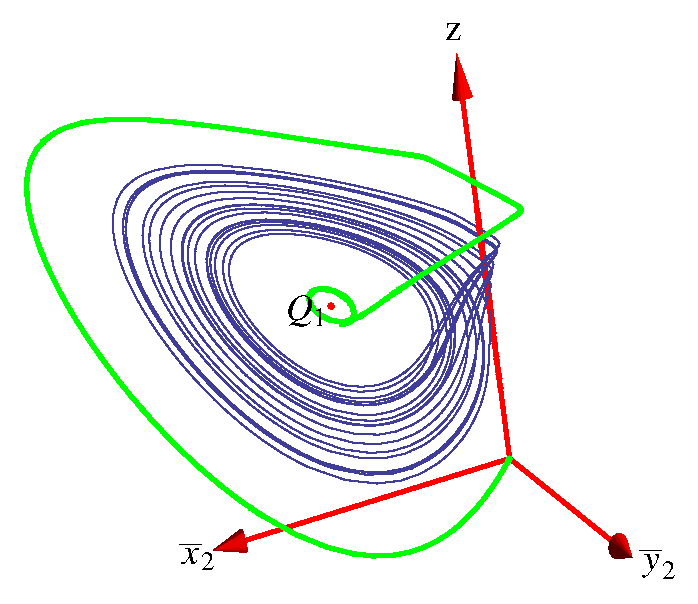
\includegraphics[width=0.35\textwidth]{../figs/CLEmfXYZ}
~~~~(\textit{b})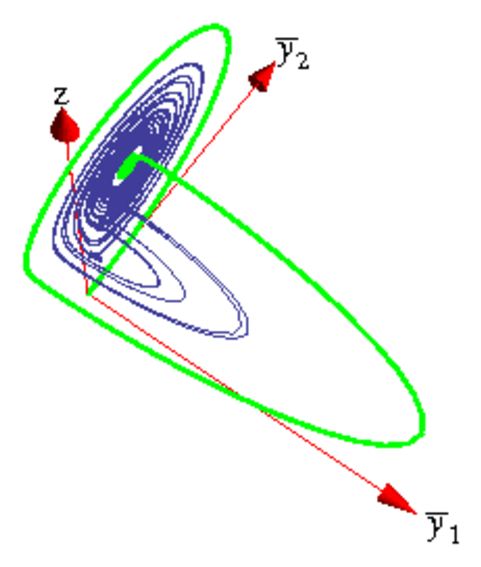
\includegraphics[width=0.35\textwidth]{../figs/CLEmfYYZ}
\end{center}
\caption{ \Statesp\
portraits of \cLe\ dynamics for $e=1/10$, $\ImrCLor=0$
in \reducedsp. Projecting on invariants given in \refeq{eq:invLaser}.
    }
\label{fig:CLEmf}
\end{figure}
%%%%%%%%%%%%%%%%%%%%%%%%%%%%%%%%%%%%%%%%%%%%%%%%%%%%%%%%%%%%%%%%

\ES{move elsewhere:
\refFig{fig:ESunrot} illustrates \mframes\ for slice fixed by
\refeq{cLeCoordSlice}.
Looks innocent, except there is nothing to
prevent a trajectory from going through $(x_1,x_2)=(0,0)$,
and what $\gSpace$ is one to use then? We can always chose a
finite time step that hops over this singularity, but in the
continuous time formulation we will not be so lucky.
}

In connection to the discussion of \refsect{s:cLeMF} note that the invariants 
are not well defined in the $x_1,\,x_2 \to 0$ limit.
Using $x=r_1\, e^{i\phi_1}\,,\, y=r_2\, e^{i\phi_2}$ we can write
\ES{dropped: for instance, $x_2 y_1-x_1 y_2 = r_1 r_2 \sin(\phi_1-\phi_2)$
and thus}
\beq
  \begin{split}
	  \overline{x}_2 &= r_1 \cont
	  \overline{y}_1 &= r_2\sin(\phi_1-\phi_2)\cont
	  \overline{y}_2 &= r_2\cos(\phi_1-\phi_2)\cont	
	  \overline{z} &= z\,.
	  \label{eq:invLaserPolar}
  \end{split}
\eeq
Therefore, for any given $y$ (therefore also for given $\phi_2$),
the limit of $\overline{y}$ for $x \rightarrow 0$
does not exist, as the above expression depends on the direction
on the complex $x$-plane along which we approach zero.

From another perspective we may say that group orbits of 
points in the $x_1=x_2=0$ subspace fail to intersect the slice
$\overline{x}_1=0,\;\overline{x}_2>0$. In \reffig{fig:CLEmf} this
becomes apparent by the trajectories in reduced space being 
stretched as they come closer to $x_1=x_2=0$ subspace where 
transverse intersection would eventually fail. In \cLe\ example no
trajectories enter the $x_1=x_2=0$ subspace, but this is a fortuitous
event\ES{point to next section after fixing discussion there.}.

It is instructive to write \cLe~\refeq{eq:CLe} in the
variables \refeq{eq:invLaser}. This is achieved by using the
chain rule \refeq{ChainRul} and expressing the result in
terms of variables \refeq{eq:invLaser}. The equations now
read
\beq
\begin{split}
\dot{\overline{x}}_1 &= 0\,\\
\dot{\overline{x}}_2 &=-\sigma  \left(\overline{x}_2-\overline{y}_2 \right)\,,\\
\dot{\overline{y}}_1 &=-\overline{y}_1- \left(e+\sigma\frac{\overline{y}_1}{\overline{x}_2} \right)\overline{y}_2\,,\\
\dot{\overline{y}}_2 &=(\RerCLor -z)\overline{x}_2+\left(e+\frac{\sigma  \overline{y}_1}{\overline{x}_2}
\right) \overline{y}_1-\overline{y}_2\,,\\
\dot{z} &=\overline{x}_2 \overline{y}_2-b z\,.
\end{split}
\eeq
We again observe the singularity as
$\overline{x}_2=r_1\rightarrow 0$.

The projections in \reffig{fig:CLEmf} let us understand the
topology of the dynamics but also present large ``jumps."
Note that the invariants \refeq{eq:invLaser} are related to
the invariant polynomials \refeq{eq:ipLaser} by division by
$\sqrt{x_1^2+x_2^2}$. This is the reason we get a clearer
visualization of the dynamics than with invariant polynomials: 
All invariants scale as the original coordinates. 
At the same time division by $\sqrt{x_1^2+x_2^2}$ causes the jumps in the
$\overline{y}$ components whenever the magnitude of $x$ comes
close to zero. 

\PublicPrivate{}{
\ES{No sure where to move this general theory on coordinate \csection s.}
Once a coordinate cross-section
$K=\{x_1=c_1,\ldots,x_r=c_N\}$ is defined by the first $N$
coordinates (relabel coordinates as necessary),
we write the group transformations as
\beq
	\overline{x}= g \cdot x = w(g,x)\,.
	\label{eq:transNorm}
\eeq
Equating the first $N$ components of the function $w$ to the
constants in the definition of the {\csection} $K_i(x)=c_i$
yields the \emph{normalization equations} for $K$:
\beq
	\overline{x}_1=w_1(g,x)=c_1,\ldots,\overline{x}_N=w_N(g,x)=c_N\,.
	\label{eq:normalization}
\eeq
The normalization equations \refeq{eq:normalization}
can always be solved\rf{FelsOlver99} for the group parameters in terms of
$x$, yielding the moving frame associated with $K$:
$\LieEl=\LieEl(x)$. Substitution of the moving frame equation back
in \refeq{eq:transNorm} will yield the $n-r$
\emph{fundamental invariants}, that is functionally independent
invariants that can be used as a basis in which any other invariant
can be expressed. Thus the fundamental invariants serve to distinguish
group orbits in the neighborhood of the {\csection}, \ie~two points
lie on the same group orbit if and only if all fundamental invariants
agree. For proof \cf~\refrefs{FelsOlver98,FelsOlver99}.

Invariants generated by \mframes\ can be used in the same manner as a Hilbert
polynomial basis for symmetry reduction, by projecting $d$-dimensional trajectories
to $(d-N)$-dimensional variables. The fact that a moving frame exists
only where group orbits have the same dimension is not as severe a restriction
as it might seem. This condition fails on a \fixedsp\ of a continuous subgroup
of \Group\ but, as we have seen in \refsect{s:symDyn}, {\fixedsp s} are flow-invariant.
Therefore, one can always hope to cover the reduced space with properly chosen {\csection s}.
Nevertheless, as we will see in next section, coordinate {\csection s} are not an optimal
choice for common actions of \SOn{2} on truncations of PDEs, such as in the \cLe\ example.
}% end PublicPrivate




% \subsection{\label{sec:CLeMF}Moving frame invariants for \cLe}




\PublicPrivate{}{
\ES{I think I might drop this part of the section, as it is a simple but
ad-hoc  modification. I will have to make sure that return map
figures are not completely elliminated from this section though.}
Geometrically we can interpret the jumps in the
$\overline{y}$ coordinates as follows: We have chosen to
measure angle on one of the irreducible subspaces of \SOn{2},
the $x$-plane, and project the dynamics on orbit space by
counter-rotating in both irreducible subspaces (the $x$- and
$y$-plane.) As long as a trajectory traces one lobe of the
Lorenz attractor the angle varies slowly and no problem
occurs. When a trajectory changes quadrant in the $x$-plane
to visit the almost opposite lobe (due to detuning we do not
visit the lobe related by rotation by $\pi$, in reality no
such thing exists) we get a rapid change in angle as the
trajectory passes close to the origin. In the $y$-plane we do
not necessarily change quadrant. Call $\Delta \theta_x$ and
$\Delta\theta_y$ the change in angle in the $x$- and
$y$-plane respectively, when the trajectory changes quadrant
in the $x$ plane. We always reduce to \reducedsp\ by
correcting by $-\Delta\theta_x$ instead of correcting by the
smallest angle.
}%end \PublicPrivate.

% Since $x$ cannot vanish
% The problem is mostly aesthetical in the present case,
% but for \KS\ system it will be important to prevent
% the denominator from vanishing.
%     \ES{Here I have a hunch that the denominator cannot
%     vanish but I can't prove it}
\PublicPrivate{}{
We observe that dynamics cannot enter $\Fix{\SOn{2}}$, \ie\
the $z$-axis, since {\fixedsp s} are flow invariant. Since
\SOn{2} representation in the \cLe\ example is a direct sum
of irreducible representations we cannot take more than one
irreducible subspace into account when setting up the
normalization equations, at least not in a convenient way. We
can however restore democracy between modes and extend
validity of the transformations to any point where the group
acts freely, by modifying the invariants as follows:
\beq
\begin{split}
	\overline{x}_2 &= (x_1^2+x_2^2)/r \cont
	\overline{y}_1 &= -(x_2 y_1-x_1 y_2)/r\cont
	\overline{y}_2 &=(x_1 y_1+x_2 y_2)/r\cont
	\overline{z} &=z\cont
	r &= \sqrt{x_1^2+x_2^2+y_1^2+y_2^2}
    \,.
	\label{eq:invLaser2}
\end{split}
\eeq
This set of invariants lacks a geometric interpretation\ES{or
does it?} but results in much cleaner phase portraits, \cf
\reffig{fig:CLEinv}.


%%%%%%%%%%%%%%%%%%%%%%%%%%%%%%%%%%%%%%%%%%%%%%%%%%%%%%%%%%%%%%%%%%
\begin{figure}[ht]
\begin{center}
  (\textit{a})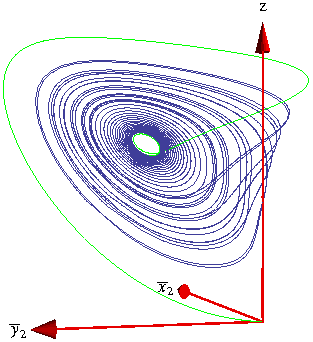
\includegraphics[width=0.35\textwidth]{../figs/CLEinvXYZ}
~~~~(\textit{b})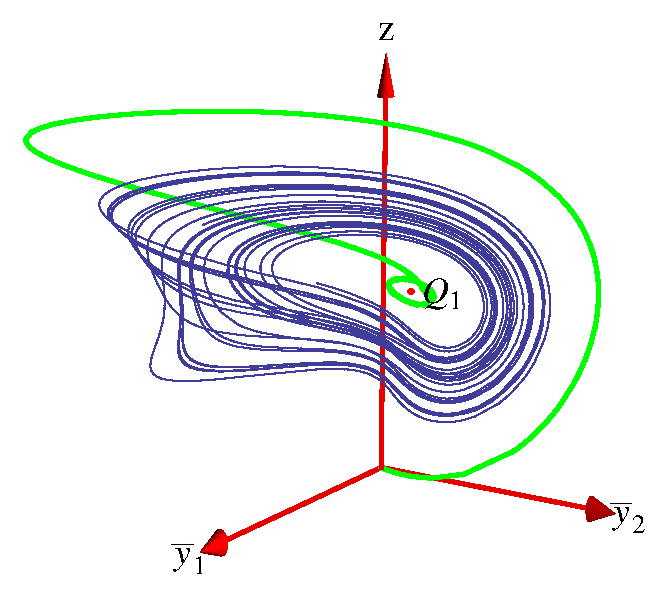
\includegraphics[width=0.35\textwidth]{../figs/CLEinvYYZ}
\end{center}
\caption{
\Statesp\ portraits of \cLe\ dynamics for $e=1/10$,
$\ImrCLor=0$ in \reducedsp. Projecting on invariants given in
\refeq{eq:invLaser2}.
    }
\label{fig:CLEinv}
\end{figure}
%%%%%%%%%%%%%%%%%%%%%%%%%%%%%%%%%%%%%%%%%%%%%%%%%%%%%%%%%%%%%%%%
\marginpar{Fetch return map figure using unmodified invariants.}

%%%%%%%%%%%%%%%%%%%%%%%%%%%%%%%%%%%%%%%%%%%%%%%%%%%%%%%%%%%%%%%%%%
\begin{figure}[ht]
\begin{center}
%   (\textit{a})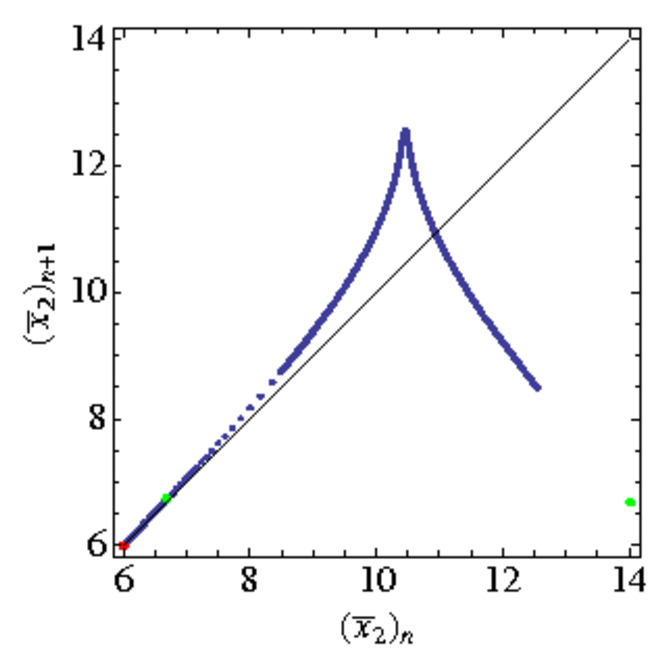
\includegraphics[width=0.35\textwidth]{../figs/CLEinvRMx2}
%  ~~~~(\textit{b})
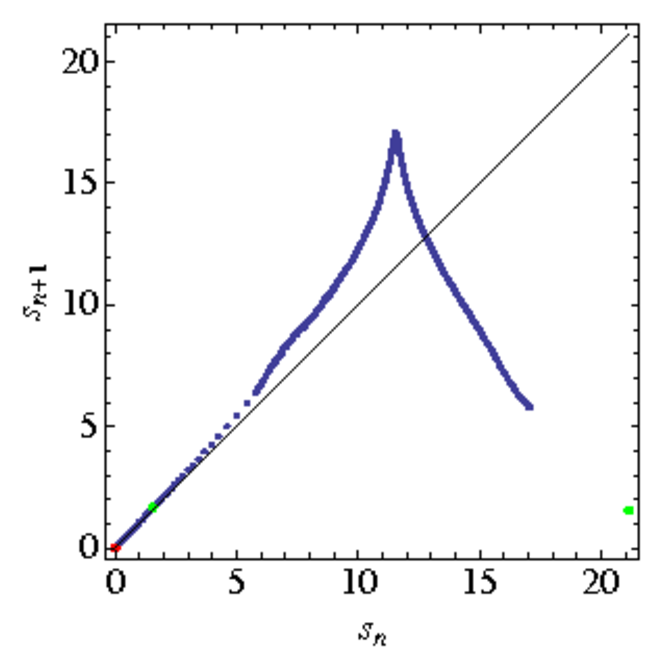
\includegraphics[width=0.35\textwidth]{../figs/CLEinvRM}
\end{center}
\caption[Return map for Complex Lorenz flow]{
Return map to the \Poincare\ surface of section
$\overline{x}_2=\overline{y}_2$ for \cLe\ with $e=1/10$,
$\ImrCLor=0$, projecting on invariants given in
\refeq{eq:invLaser2}. The return map coordinate is the
Euclidean length along the \Poincare\ section of the unstable
manifold of $E_1$.
    }
\label{fig:CLEinvRM}
\end{figure}
%%%%%%%%%%%%%%%%%%%%%%%%%%%%%%%%%%%%%%%%%%%%%%%%%%%%%%%%%%%%%%%%
} %end PublicPrivate
